\documentclass[a4paper]{article}
\usepackage[document]{ragged2e}
\usepackage{fontspec}
\usepackage{geometry}
\usepackage{graphicx}
\usepackage{url}
\usepackage{minted}
\usepackage{pdfpages}
\geometry{left=2cm}
\geometry{right=2cm}
\geometry{top=2cm}
\geometry{bottom=2cm}
\setmainfont{Liberation Serif}
\setmonofont[Scale=0.8]{Hack}
\sloppy

\setlength{\parindent}{0pt}
\setlength{\tabcolsep}{10pt}
\renewcommand*{\arraystretch}{2}
\renewcommand{\theFancyVerbLine}{\textbf{\arabic{FancyVerbLine}}}

\setminted{
  linenos,
  breaklines,
  breakanywhere,
  breaksymbolleft=,
  fontsize=\fontsize{9}{9}\selectfont,
  numbersep=5pt,
}
\usemintedstyle{emacs}

\graphicspath{ {./pics/} }

\begin{document}
  \fontsize{14}{16}\selectfont

  \begin{titlepage}
    \begin{minipage}{0.2\textwidth}
      
\includegraphics[scale=0.4]{logo}
    \end{minipage}
    \begin{minipage}{0.7\textwidth}\centering
      \fontsize{10}{12}\selectfont
      \textbf{
        Федеральное государственное бюджетное образовательное учреждение \\
        высшего профессионального образования \\
        «Московский государственный технический университет имени Н.Э. Баумана» \\
        (МГТУ им. Н.Э. Баумана)
      }
    \end{minipage}

    \vspace{5cm}
    \centering
    \textbf{
      Лабораторная работа 6 \\
      по курсу «Технологии машинного обучения» \\
    }

    \vspace{5cm}
    \begin{flushright}
    Выполнил \\
    студент группы ИУ5-64 \\
    XXX
    \end{flushright}
    \vspace*{\fill}
    Москва, 2021
  \end{titlepage}

  \section*{Цель работы}
  изучение возможностей демонстрации моделей машинного обучения с помощью веб-приложений.

  \section*{Задание}
  Разработайте макет веб-приложения, предназначенного для анализа данных. \\
  Вариант 1. Макет должен быть реализован для одной модели машинного обучения. Макет должен позволять: \\
  \begin{itemize}
    \item задавать гиперпараметры алгоритма,
    \item производить обучение,
    \item осуществлять просмотр результатов обучения, в том числе в виде графиков.
  \end{itemize}
  Вариант 2. Макет должен быть реализован для нескольких моделей машинного обучения. Макет должен позволять:
  \begin{itemize}
    \item выбирать модели для обучения,
    \item производить обучение,
    \item осуществлять просмотр результатов обучения, в том числе в виде графиков.
  \end{itemize}

  \section*{Код}
  \inputminted{python}{6.py}

  \section*{Результат работы}
  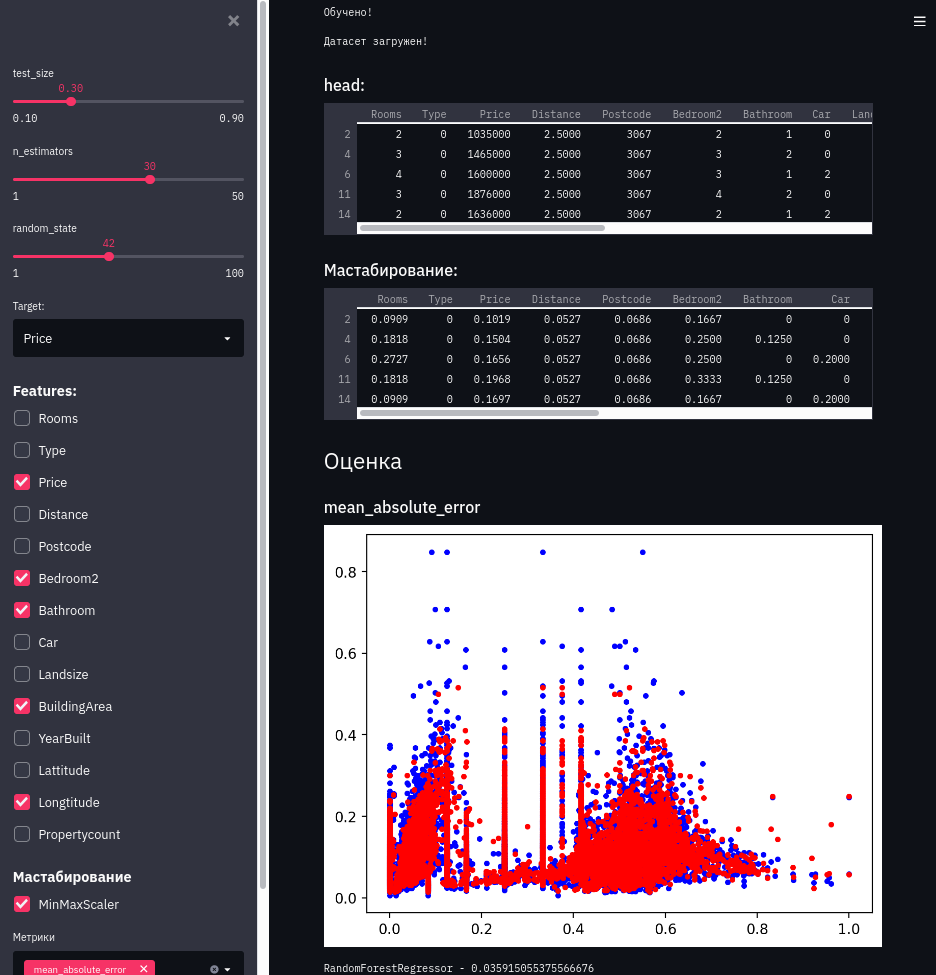
\includegraphics[scale=0.5]{scr}
\end{document}
